\documentclass[homework]{IEEEtran}
\IEEEoverridecommandlockouts
% The preceding line is only needed to identify funding in the first footnote. If that is unneeded, please comment it out.
\usepackage{cite}
\usepackage{CJKutf8}
\usepackage{indentfirst}
\usepackage{amsmath,amssymb,amsfonts}
\usepackage{algorithmic}
\usepackage{graphicx}
\usepackage{textcomp}
\usepackage{xcolor}
\usepackage{hyperref}
\usepackage[justification=centering]{caption}
\setlength{\parindent}{2em}
\def\BibTeX{{\rm B\kern-.05em{\sc i\kern-.025em b}\kern-.08em
    T\kern-.1667em\lower.7ex\hbox{E}\kern-.125emX}}
\begin{document}

\title{Homework of Pattern classification IV\\
{\footnotesize \textsuperscript{*}Name: Xue Yuan  | Student number: 202228015926034}
}

\author{}
\maketitle

\begin{abstract}
This document is about the first homework for Pattern classification by \LaTeX.
\end{abstract}

\section{Short Answers and Descriptions}
\begin{CJK}{UTF8}{gkai}
$\mathbf{Q1}$: 请描述使用高斯混合模型进行数据聚类的过程。 \par
$\mathbf{A}$: 采用gauss混合模型进行聚类,其主要包括三个过程:
\begin{enumerate}
\item 样本的生成:通过类先验概率密度$p(\omega_j)$随机选择一个样本类别,
然后通过类条件概率密度函数$p(x\vert\omega,\theta_j)$随机生成相应的样本。其中,高斯混合模型GMM(Gaussian Mixture Model)的概率函数为:
\begin{align}
P(y \vert \theta) &= \sum \limits_{k=1}^{k} \alpha_k \varphi(y \vert \theta_k) \\
\sum \limits_{k=1}^{k} \alpha_k &=1; \alpha_k \geq 0 \\
\varphi(y \vert \theta_k) &= \frac{1}{\sqrt{2 \pi} \sigma_k} \exp \left(-\frac{(y- \mu_k)^2}{2 \sigma_{k}^{2}}\right)
\end{align}
\item 我们认为:样本来自c个不同类别,c的值是已知的。每一类的先验概率$p(\omega_j)$也是已知的,
类条件概率密度函数$p(x\vert\omega,\theta_j)$形式上是已知的,存在c个参数向量$\theta_j,j = 1,2,\dots,c$。
\item 根据极大似然估计,求解类条件概率密度函数中的参数$\theta_j$,再根据最大后验概率进行聚类划分:
$$
C(\mathbf{x})=\arg \max _{j} p\left(\omega_{j} \mid \mathbf{x}, \boldsymbol{\theta}\right)
$$
后验概率:
$$
p\left(\omega_{j} \mid \mathbf{x}, \boldsymbol{\theta}\right)=\frac{p\left(\mathbf{x} \mid \omega_{j},
 \boldsymbol{\theta}\right) P\left(\omega_{j}\right)}{\sum\limits_{i=1}^{c} p\left(\mathbf{x} \mid \omega_{i}, \boldsymbol{\theta}\right) P\left(\omega_{i}\right)}
$$
\end{enumerate}

$\mathbf{Q2}$:对于:$x_1=(4,5)^T,x_2=(1,4)^T,x_3=(0,1)^T,x_4=(5,0)^T,x_5=(4,1)^T,x_6=(0,6)^T$现有以下三种聚类划分。\par
\begin{figure}[htb]
    \centerline{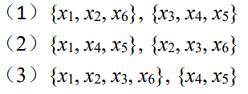
\includegraphics{Images/fig1.png}}
    \caption{Three types of division}
    \label{fig1}
    \end{figure}
假定我们聚类的准则是最小平方和误差,请判断上述三个划分中哪个更好?\par
$\mathbf{A}$:由最小平方和误差定义,可以计算各个划分相应的误差大小为$tr\left[S_w \right]$,其中,$S_w$为:
\begin{align*}
\mathbf{S}_{W}&=\sum_{i=1}^{c} \sum_{\mathbf{x} \in \mathcal{D}_{i}}\left(\mathbf{x}-\mathbf{m}_{i}\right)\left(\mathbf{x}-\mathbf{m}_{i}\right)^{t} \\
    &=\sum_{k=1}^{6} \mathbf{x}_{k} \mathbf{x}_{k}^{t}-\sum_{i=1}^{c} n_{i} \mathbf{m}_{i} \mathbf{m}_{i}^{t}
\end{align*}
容易计算:
$$
\sum_{k=1}^{6} \mathbf{x}_{k} \mathbf{x}_{k}^{t} = 
\left(\begin{array}{ll}58 & 28 \\ 28 & 94\end{array}\right)
$$ 
计算三种聚类划分
$$
\mathbf{m}_{i}=\frac{1}{n_{i}} \sum_{\mathbf{x} \in \mathcal{D}_{i}} \mathbf{x}
$$
\begin{enumerate}
    \item 第一种划分的聚类中心为:
    $$
    m_1 = \frac{1}{3} \left(
    \begin{pmatrix}4 \\ 5\end{pmatrix}+\begin{pmatrix}1 \\ 4\end{pmatrix}+\begin{pmatrix}0 \\ 6\end{pmatrix} \right)
    = \begin{pmatrix}5/3 \\ 5\end{pmatrix}
    $$

    $$
    m_2 = \frac{1}{3} \left(
    \begin{pmatrix}0 \\ 1\end{pmatrix}+\begin{pmatrix}5 \\ 0\end{pmatrix}+\begin{pmatrix}4 \\ 1\end{pmatrix} \right)
    = \begin{pmatrix}3 \\ 2/3\end{pmatrix}
    $$
    可以计算:
$$
\sum_{i=1}^{c} n_{i} \mathbf{m}_{i} \mathbf{m}_{i}^{t} = 3\left(m_1m_{1}^T+m_2m_{2}^T\right)
=
\begin{pmatrix}106 / 3 & 31\\ 31 & 229 /3\end{pmatrix}
$$

$$
S_{w1} = \begin{pmatrix}58 & 28 \\28 & 94\end{pmatrix}-\begin{pmatrix}106 / 3 & 31\\ 31 & 229 /3\end{pmatrix}
=\begin{pmatrix}68 / 3 & -3\\ -3 & 53 /3\end{pmatrix}
$$
可以得到:$tr\left[S_{w1} \right] = 121/3 = 40.33$
\item 第二种划分的聚类中心为:
$$
 m_1 = \frac{1}{3} \left(
\begin{pmatrix}4 \\ 5\end{pmatrix}+\begin{pmatrix}5 \\ 0\end{pmatrix}+\begin{pmatrix}4 \\ 1\end{pmatrix} \right)
= \begin{pmatrix}13/3 \\ 2\end{pmatrix}
$$

$$
m_2 = \frac{1}{3} \left(
\begin{pmatrix}1 \\ 4\end{pmatrix}+\begin{pmatrix}0 \\ 1\end{pmatrix}+\begin{pmatrix}0 \\ 6\end{pmatrix} \right)
= \begin{pmatrix}1/3 \\ 11/3\end{pmatrix}
$$
同理可以计算:
$$
\sum_{i=1}^{c} n_{i} \mathbf{m}_{i} \mathbf{m}_{i}^{t} = 
\begin{pmatrix}170/3 & 89/3\\ 89/3 & 157/3
\end{pmatrix}
$$

$$
S_{w2} = \begin{pmatrix}58 & 28 \\28 & 94\end{pmatrix}-\begin{pmatrix}170/3 & 89/3\\ 89/3 & 157/3\end{pmatrix}
=\begin{pmatrix}4/3 & -5/3\\ -5/3 & 125/3\end{pmatrix}
$$
可以得到:$tr\left[S_{w2} \right] = 43$
\item 第三种划分的聚类中心为:
$$
 m_1 = \frac{1}{4} \left(
\begin{pmatrix}4 \\ 5\end{pmatrix}+\begin{pmatrix}1 \\ 4\end{pmatrix}+\begin{pmatrix}0 \\ 1\end{pmatrix}+\begin{pmatrix}0 \\ 6
\end{pmatrix} \right)
= \begin{pmatrix}5/4 \\ 4\end{pmatrix}
$$

$$
m_2 = \frac{1}{2} \left(
\begin{pmatrix}5 \\ 0\end{pmatrix}+\begin{pmatrix}4 \\ 1\end{pmatrix} \right)
= \begin{pmatrix}9/2 \\ 1/2\end{pmatrix}
$$
同理可以计算:
$$
\sum_{i=1}^{c} n_{i} \mathbf{m}_{i} \mathbf{m}_{i}^{t} = \begin{pmatrix}187/4 & 49/2\\ 49/2 & 129/2\end{pmatrix}
$$

$$
S_{w3} = \begin{pmatrix}58 & 28 \\28 & 94\end{pmatrix}-\begin{pmatrix}187/4 & 49/2\\ 49/2 & 129/2\end{pmatrix}
=\begin{pmatrix}45/4 & 7/2\\ 7/2 & 59/2\end{pmatrix}
$$
可以得到:$tr\left[S_{w3} \right] = 163/4 = 40.75$
\end{enumerate}
综上计算可以看出:
$$
tr[S_{w2}] = 43 > tr[S_{w3}] = 40.75 > tr[S_{w1}] = 40.33
$$
因此,根据最小平方和误差准则,可以认定:第一种分类方法最为合理。 \par
$\mathbf{Q3}$:请阐述$k-means$聚类和模糊$k-means$聚类的异同。\par
$\mathbf{A1}$:相同之处在于,这两种方法都需要预设类别种类数,需要预设初始化各个类别的聚类中心,并不断迭代跟新聚类中心。
并且它们都是通过误差平方和准则的方法不断迭代修正。因此,这两种方法都对初始化条件敏感,且难以处理外点。\par
$\mathbf{A2}$:不同之处在于,模糊$k-means$聚类认为样本以一定概率隶属于不同类别(称隶属度),并由此修正了误差平方和准则的表达形式如下:
$$
J_{fuz} = \sum\limits_{i=1}^{c} \sum\limits_{j=1}^{n}\left[\mu_i (x_j)\right]^b \rVert x_j - m_i \rVert ^2
$$ \par
因此,每一次的迭代不仅要跟新聚类中心,还要对隶属度进行更新,最终使聚类中心和隶属度的变化量都小于可接受极限。
相应的输出量同样包括聚类中心和样本属于它们的隶属度。 \par
$\mathbf{A3}$:最优解的推导过程如下,由优化目标函数:
$$
\begin{array}{l}
    \min _{\mu, m} \sum\limits_{i=1}^{c} \sum\limits_{j=1}^{n}\left[\mu_{i}\left(\mathbf{x}_{j}\right)\right]^{b}\left\|\mathbf{x}_{j}-\mathbf{m}_{i}\right\|^{2} \\
    \\
    \text { s.t. } \sum\limits_{i=1}^{c} \mu_{i}\left(\mathbf{x}_{j}\right)=1, \quad j=1,2, \ldots, n
    \end{array}
$$
可以引入n个拉格朗日因子:
$$
J^{\prime}=\sum\limits_{i=1}^{c} \sum\limits_{j=1}^{n} [\mu_i (x_j)]^{b}\left\|\mathbf{x}_{j}-\mathbf{m}_{i}\right\|^{2}
    +\sum\limits_{j=1}^{n} \lambda_{i}\left(\sum_{i=1}^{c} [\mu_i (x_j)]^{b}-1\right)
$$ \par
欲使J最小化,可以分别使之对聚类中心$m_k$和隶属度$\mu_i (x_j)$求偏导。
对聚类中心,我们记,$\mu_i (x_j) = \mu_{ij}$,可得:
$$
\frac{\partial J^{\prime}}{\partial m_{k}}=\sum_{i=1}^{c} \sum_{j=1}^{n} \frac{\partial \mu_{i j}^{b}\left\|\mathbf{x}_{j}-\mathbf{m}_{i}\right\|^{2}}
{\partial m_{i}}-\frac{\partial}{\partial m_{k}} \sum_{j=1}^{n} \lambda_{j}\left(\sum_{i=1}^{c} \mu_{i j}-1\right)
$$ \par
注意到:
$$
\sum\limits_{i=1}^{c} \mu_{i}\left(\mathbf{x}_{j}\right)=1, \quad j=1,2, \ldots, n
$$
则:
\begin{align*}
    \frac{\partial J^{\prime}}{\partial m_{k}} &= \sum_{i = 1}^{c} \sum_{j = 1}^{n} \frac{\partial \mu_{i j}^{b}\left\|\mathbf{x}_{j}-\mathbf{m}_{i}\right\|^{2}}{\partial m_{k}} \\ 
    &= \sum_{i = 1}^{c} \sum_{j = 1}^{n} \mu_{i j}^{b} \frac{\partial}{\partial m_{k}}\left\|\mathbf{x}_{j}-\mathbf{m}_{i}\right\|^{2} \\ 
    &= \sum_{j = 1}^{n} \mu_{k j}^{b} \frac{\partial}{\partial m_{k}}\left\|\mathbf{x}_{j}-\mathbf{m}_{k}\right\|^{2} \\ 
    &= -2 \sum_{j = 1}^{n} \mu_{k j}^{b}\left(x_{j}-m_{k}\right) = 0 
\end{align*}
改换下标$k=i$,化简得到聚类中心的优化结果表达式:
$$
\mathbf{m}_{i}=\frac{\sum\limits_{j=1}^{n}\left[\mu_{i}\left(\mathbf{x}_{j}\right)\right]^{b} \mathbf{x}_{j}}{\sum\limits_{j=1}^{n}\left[\mu_{i}\left(\mathbf{x}_{j}\right)\right]^{b}}
$$ \par
对隶属度$\mu_{i}\left(\mathbf{x}_{j}\right)$(以下简写$\mu_{ij}$)求偏导,可以采用分部分求导的策略,对表达式左侧求导有:
$$
\frac{\partial J^{\prime}}{\partial \mu_{i j}}=\frac{\partial}{\partial \mu_{i j}} \sum_{j=1}^{n} \sum_{i=1}^{c} \mu_{i j}^{b}\left\|\mathbf{x}_{j}-\mathbf{m}_{i}\right\|^{2}
$$
不妨记:$d_{ij}=\left(x_j - m_i\right)$,有:
$$
\frac{\partial J^{\prime}}{\partial \mu_{i j}}=\sum_{j=1}^{n} \sum_{i=1}^{c} \frac{\partial}{\partial \mu_{i j}} \mu_{i j}^{b} d_{i j}=\sum_{j=1}^{n} \sum_{i=1}^{c} b \mu_{i j}^{b-1} d_{i j}
$$ \par
对表达式右侧求导有:
\begin{align*}
    \frac{\partial J^{\prime}}{\partial \mu_{i j}} &=\frac{\partial}{\partial \mu_{i j}} \sum_{j=1}^{n} \lambda_{j}\left(\sum_{i=1}^{c} \mu_{i j}-1\right) \\
     &=\frac{\partial}{\partial \mu_{i j}} \sum_{j=1}^{n}\left(\sum_{i=1}^{c} \lambda_{j} \mu_{i j}-\lambda_{j}\right) \\
     &=\sum_{j=1}^{n} \sum_{i=1}^{c} \frac{\partial}{\partial \mu_{i j}} \lambda_{j} \mu_{i j} \\
     &=\sum_{j=1}^{n} c \lambda_{j}
\end{align*} \par
合并两侧求导结果,可得:
\begin{align*}
\frac{\partial J^{\prime}}{\partial \mu_{i j}} &= \sum_{j=1}^{n} \sum_{i=1}^{c} b \mu_{i j}^{b-1} d_{i j} + \sum_{j=1}^{n} c \lambda_{j} \\
        &=\sum_{j=1}^{n}\left(\sum_{i=1}^{c} b \mu_{i j}^{b-1} d_{i j}+c \lambda_{j}\right) \\
        &=\sum_{j=1}^{n}\sum_{i=1}^{c}\left(b \mu_{i j}^{b-1} d_{i j}+\lambda_{j}\right) = 0
\end{align*} \par
考虑初始条件:
\begin{align*}
         b \mu_{i j}^{b-1} d_{i j}+\lambda_{j} &\geq 0 \\
    \therefore b \mu_{i j}^{b-1} d_{i j}+\lambda_{j}&=0, \forall i=1 \dots c
\end{align*} \par
可以化简:
$$
\mu_{i j}=\left(\frac{-\lambda_{j}}{b d_{i j}}\right)^{\frac{1}{b-1}}
$$ \par
考虑到:
$$
\sum_{k=1}^{c} \mu_{k j}=1 \quad \forall j=1, \ldots, n
$$ \par
可以计算:
\begin{align*} 
\sum_{k=1}^{c}\left(\frac{-\lambda_{j}}{b d_{k j}}\right)^{\frac{1}{b-1}} &=\left(\frac{-\lambda_{j}}{b}\right)^{\frac{1}{b-1}} \sum_{k=1}^{c}\left(\frac{1}{d_{k j}}\right)^{\frac{1}{b-1}}=1 \\
\Rightarrow\left(\frac{-\lambda_{j}}{b}\right)^{\frac{1}{b-1}} &=\frac{1}{\sum\limits_{k=1}^{c}\left(\frac{1}{d_{k j}}\right)^{\frac{1}{b-1}}}
\end{align*} \par
带回到$\mu_{ij}$表达式中,化简可得:
$$
\mu_{i j}=\frac{1}{\sum_{k=1}^{c}\left(\frac{1}{d_{k j}}\right)^{\frac{1}{m-1}}} \cdot\left(\frac{1}{d_{i j}}\right)^{\frac{1}{m-1}}
$$ \par
带入$d_{ij}=\left(x_j - m_i\right)$,可以得到最终的隶属度优化结果表达式:
$$
\mu_{i}\left(\mathbf{x}_{j}\right)=\frac{\left(1 / \left\|\mathbf{x}_{j}-\mathbf{m}_{i}\right\|^{2}\right)^{1 /(b-1)}}{\sum\limits_{k=1}^{c}\left(1 /\left\|\mathbf{x}_{j}-\mathbf{m}_{k}\right\|^{2}\right)^{1 /(b-1)}}
$$ \par
$\mathbf{Q4}$: 证明:在 K 均值聚类中,在某次迭代的时候,将属于第 i 类的样本点移到第 j 类之后,
属于第 i 类的样本点对应的误差平方和将变为: \par
$$
J_{i}^{*} = J_i - \frac{n_i \Vert \hat{x}-m_i\Vert^{2}}{n_i - 1}
$$ \par
$\mathbf{A}$: 由类中心变化:
$$
m_{i}^{*} = m_i - \frac{\hat{x}-m_j}{n_i-1}
$$ \par
则此时的误差平方和可以表示为:
\begin{align*}
 J_{i}^{*} &= \sum\limits_{x\in D_i} \Vert x-m_{i}^{*} \Vert^{2} - \Vert \hat{x}-m_{i}^{*} \Vert^{2}	\\
	&=\sum\limits_{x\in D_j} \left(\Vert x-m_i \Vert^{2}+\frac{2}{n_i-1}(\hat{x}-m_i)^{T}(x-m_i) \right) \\
    &+\sum\limits_{x\in D_j} \frac{\Vert \hat{x}-m_i\Vert^{2}}{(n_i-1)^2} -\Vert \frac{n_i}{n_i-1} \left(\hat{x}-m_i \right) \Vert^{2}  \\
	&=J_i + \frac{2}{n_i-1}(\hat{x}-m_i)^{T}\left(\sum\limits_{x\in D_i}x-\sum\limits_{x\in D_i}m_i\right) \\
    &+\left[\frac{n_i \Vert \hat{x}-m_i\Vert^{2}}{(n_i-1)^2} - \frac{n_{i}^{2} \Vert \hat{x}-m_i\Vert^{2}}{(n_i-1)^2}\right]	\\
	&= J_i + \frac{2}{n_i-1}(\hat{x}-m_i)^{T}\left(n_i m_i - n_i m_i\right)-\frac{n_i \Vert \hat{x}-m_i\Vert^{2}}{(n_i-1)} \\
	&=J_i - \frac{n_i \Vert \hat{x}-m_i\Vert^{2}}{(n_i-1)}
\end{align*}\par
综上,可以得到属于第$i$类的样本点引起的误差平方和的减小n量为:
\begin{align*}
J_{i}^{*} &= \sum\limits_{x\in D_i} \Vert x-m_{i}^{*} \Vert ^{2} - \Vert \hat{x} -m_{i}^{*} \Vert^{2}
  &=J_i - \frac{n_i \Vert \hat{x}-m_i\Vert^{2}}{n_i - 1}
\end{align*}\par
$\mathbf{Q5}$:
$\mathbf{A1}$:原问题为:
\begin{align*}
    \min_{w,b}\frac{1}{2} \Vert w \Vert^{2} &+ C\sum\limits_{i=1}^{N}\xi_i \\
    s.t. \quad y_i\left( w^Tx_i+b\right) &\geq 1-\xi_i, i=1,2\dot,N \\
    \xi_i \geq 0, i &= 1,2,\dot,N
\end{align*}\par
引入拉格朗日乘子,得到拉格朗日函数:
$$
L\left(w,b,\xi,\alpha,\mu\right)=\frac{1}{2}\Vert w\Vert^{2} +C\sum\limits_{i=1}^{N}\xi_i+
$$
$$
\sum\limits_{i=1}^{N}\alpha_i \left( 1-\xi_i-y_i\left(w^Tx_i+b\right) \right) -\sum\limits_{i=1}^{N}\mu_i \xi_i
$$\par
可以得到原问题的对偶问题:
\begin{align*}
\max_{\alpha} \min_{w,b}&L\left( w,b,\xi,\alpha,\mu \right) \\
s.t. \quad \alpha_i &\geq 0,\quad \mu_i \geq 0
\end{align*}\par
$\mathbf{A2}$:如图$Fig2$所示,当C取值很大时($C\to +\infty$时,线性支持向量机退化为线性可分的支持向量机),SVM更加关注分类准确度,因此其分界面间隔很小,基本没有错分现象出现;
同样,当C取值很小甚至接近于0时,SVM更加关注分类间隔问题,倾向于产生尽量大的分类间隔,从而产生小部分错分点。
\begin{figure}[htb]
    \centerline{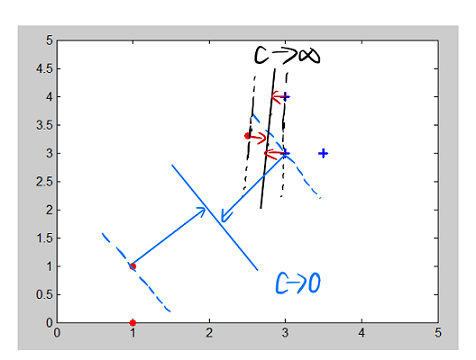
\includegraphics{Images/fig2.png}}
    \caption{Segmentation Surface under Different C Values}
    \label{fig2}
    \end{figure}

$\mathbf{Q6}$:分别阐述线性可分向量机中的支持向量的几何意义和代数意义。\par
$\mathbf{A1}$:从图像上出发,线性可分向量机的支持向量对应的是关于分割面等距的、最近的且在不错分前提下使得类间的几何距离相对最大的这样一批样本点。\par
$\mathbf{A2}$:从代数上出发,对于线性可分样本,支持向量是指的使下列等式成立(约束条件)的样本点:
\begin{equation*}
    \begin{cases}
        w^Tx_i+b=-1, &y_i=-1 \\
        w^Tx_i+b=1,&y_i=1 
    \end{cases}
\end{equation*}\par
合并得到:
$$
y_i\left(w^Tx_i+b \right) = 1
$$\par
引入拉格朗日函数后,解决对偶问题所引出的约束条件如下,使得该条件成立的样本点便称作支持向量:
$$
\alpha_{i}^{*} \geq 0,\quad y_i\left(w^{*T}x_i+b^{*} \right) = 1
$$\par
$\mathbf{Q7}$:结合图例,阐述线性可分支持向量机中的分类间隔的含义 \par
\begin{figure}[htb]
    \centerline{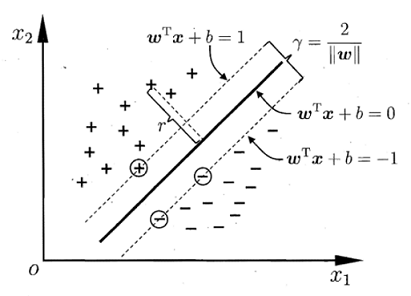
\includegraphics{Images/fig3.png}}
    \caption{Classification Interval of Linear Separable Vector Machines}
    \label{fig3}
    \end{figure}
$\mathbf{A}$:对线性可分支持向量机,如上图所示,分类间隔描述了两类样本点集被分类面分隔开后,两类样本点与分类面之间的间隙大小和,即图中虚线间隙距离。从代数上,其实就是下式:
$$
\gamma = \frac{2}{\Vert w \Vert_{2}}
$$
我们的初始优化目标就是使分类间隔即得该式取得最大值。\par
$\mathbf{Q8}$:请描述使用交叉验证对线性支持向量机的参数C进行设置的过程	。	\par
$\mathbf{A}$:交叉验证方法本质上就是划分部分样本作为验证集(validation),以实现对训练参数不断快速优化的过程。如下图所示:
\begin{figure}[htb]
    \centerline{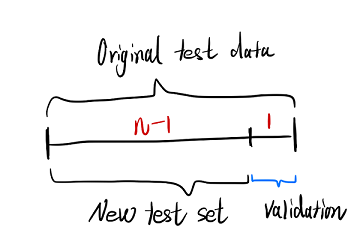
\includegraphics{Images/fig4.png}}
    \caption{Cross-Validation Diagram}
    \label{fig4}
    \end{figure}
\begin{enumerate}
	\item 将原训练集划分为n份,随机取其中$n-1$份样本做为训练集训练分类器(SVM模型),剩下的一份样本作为验证集(validation),用来测试训练成果。
	\item 取不同C值并不断重复1)中过程,取正确率最高的参数值作为C值。
	\item 将2)部筛选出的C值最为参数值,在所有训练样本上重新学习SVM模型,获得相应的模型参数。
\end{enumerate}\par
$\mathbf{Q9}$:	将支持向量机对应的优化问题进行对偶化之后,有什么优势?\par
$\mathbf{A}$:进行对偶化操作后,可以使得优化问题更容易求解,原问题的优化是一个二次规划问题,求解较麻烦,用拉格朗日乘子法转换后可以用smo等算法更简单地优化。  \par
并且对偶化操作后,更加容易引入核函数,可以推广到非线性分类问题的求解。由于转换后的假设函数主要由内积运算构成,可以使用核函数简化特征映射到高维空间后的内积运算,高效地求解非线性问题。

\end{CJK}

\vspace{10mm}
\section{Programming}
\begin{CJK}{UTF8}{gkai}

$\mathbf{Q1}$:对如下的 30 个数据进行 K-均值聚类,聚类个数设置为 K=4 \par
\begin{enumerate}
	\item 指出所使用的初始聚类中心,并报告在此条件下得到的最终聚类结果以及需要的迭代次数,对应的误差平方和。
	\item 重新选择 3 组不同的初始聚类中心,给出对应的聚类结果和误差平方和。
\end{enumerate}\par

$\mathbf{A1}$:我们采用了基于$Python3.9$的模块化设计,代码均由$Python$编译。初始的聚类中心由程序随机筛选得出,程序运行的结果图如下图所示: \par
随机取得的初始聚类中心为:
\begin{figure}[htb]
    \centerline{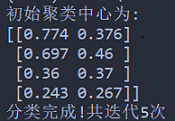
\includegraphics{Images/fig5.png}}
    \caption{Initial Cluster Center}
    \label{fig5}
    \end{figure} \par

初始分布情况为: \par
\begin{figure}[htb]
    \centerline{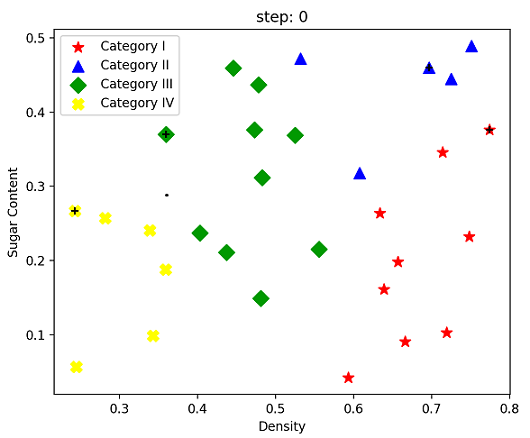
\includegraphics{Images/fig6.png}}
    \caption{Initial Situation}
    \label{fig6}
    \end{figure} 

\begin{figure}[htb]
    \centerline{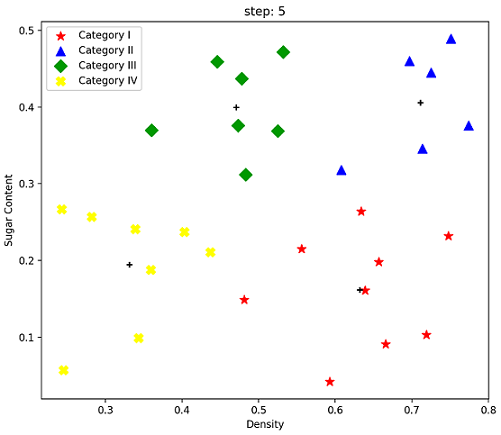
\includegraphics{Images/fig7.png}}
    \caption{Final Clustering Results}
    \label{fig7}
    \end{figure} \par
最终聚类的结果为如上图所示。可见,共需迭代5次,相应的最终聚类结果数据和误差平方和如图$Fig9$所示: \par
\begin{figure}[htb]
    \centerline{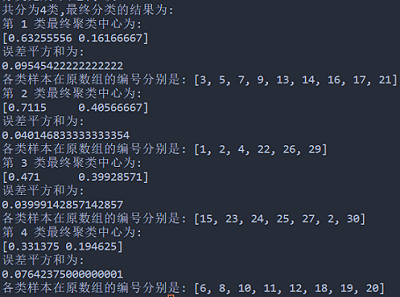
\includegraphics{Images/fig8.png}}
    \caption{Final clustering Results[numerical value]}
    \label{fig8}
    \end{figure} \par
$\mathbf{A2}$:随机选取不同的聚类中心数据如下:     \par
\begin{figure}[htb]
    \centerline{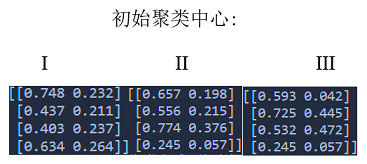
\includegraphics{Images/fig9.png}}
    \caption{Three groups of different initial cluster centers}
    \label{fig9}
    \end{figure} \par

\vspace{15mm}
他们最终的聚类结果由图$fig10 \sim fig12$展示,具体的运行结果反映在附录中。 \par
\begin{figure}[htb]
    \centerline{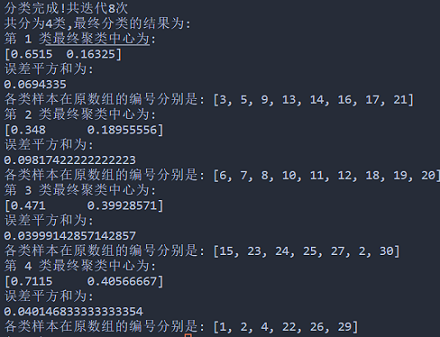
\includegraphics{Images/fig10.png}}
    \caption{Final clustering Results[Group I]}
    \label{fig10}
    \end{figure} \par
\begin{figure}[htb]
    \centerline{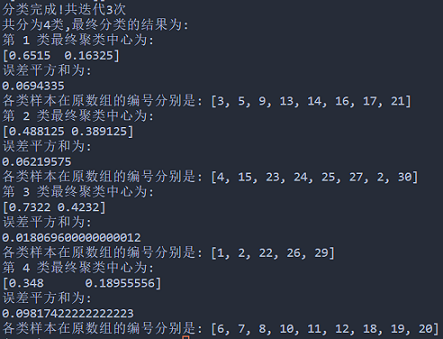
\includegraphics{Images/fig11.png}}
    \caption{Final clustering Results[Group II]}
    \label{fig11}
    \end{figure} \par
\begin{figure}[htb]
    \centerline{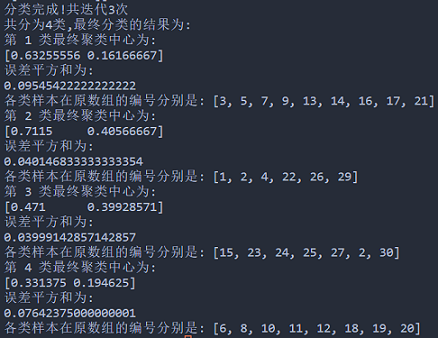
\includegraphics{Images/fig12.png}}
    \caption{Final clustering Results[Group III]}
    \label{fig12}
    \end{figure} \par

\clearpage
$\mathbf{Q2}$:对上述数据集进行模糊 K-均值聚类,聚类个数设置为 K=4。指出使用的初始聚类中心、
初始隶属度,报告在此初始化条件下的聚类结果(即:样本属于不同聚类的隶属度)以及需要的迭代次数 \par
$\mathbf{A}$:我们设定,当隶属度矩阵各个向量变化小于$\epsilon=1e^-7$时,终止迭代。
随机初始化的聚类中心由下图(限于篇幅,初始隶属度数据在附录中展示)给出: 
\begin{figure}[htb]
    \centerline{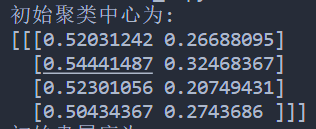
\includegraphics{Images/fig13.png}}
    \caption{Initial data [Fuzzy K-means]}
    \label{fig13}
    \end{figure} \par
最终分类结果如$Fig14$所示,可以看出,程序共进行了28次的迭代:
\begin{figure}[htb]
    \centerline{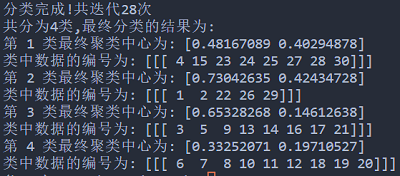
\includegraphics{Images/fig14.png}}
    \caption{Final clustering Results[Fuzzy K-means]}
    \label{fig14}
    \end{figure} \par
初始的分类图像:
\begin{figure}[htb]
    \centerline{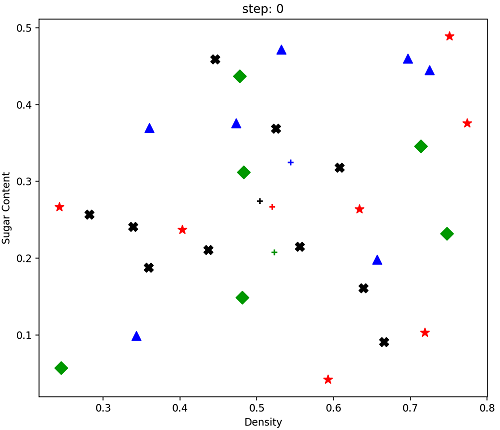
\includegraphics{Images/fig15.png}}
    \caption{Initial Situation}
    \label{fig15}
    \end{figure} \par
\newpage
最终的分类情况:
\begin{figure}[htb]
    \centerline{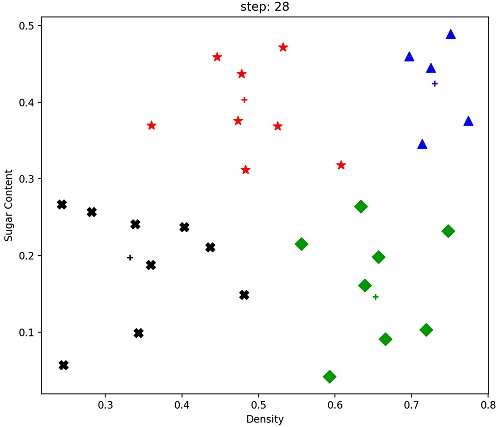
\includegraphics{Images/fig16.png}}
    \caption{Final Clustering Situation}
    \label{fig16}
    \end{figure} \par

$\mathbf{Thinking}$:事实上,当程序迭代至$Step 8$次时,聚类中心和样本隶属度虽然还在变化,
但变化幅度过小,导致样本分布(几乎)不发生变化,赝本隶属情况事实上已经不再更新。后续的计算虽然
可以在一定程度上精进参数准确度,但对于实际问题的解决几乎没有作用,浪费了算力。 \par
调节初始参数和收敛条件$\epsilon$值大小或许可以优化这一问题。
\end{CJK}

\clearpage

\section{Appendix}
\begin{CJK}{UTF8}{gkai}
    本次作业中,所采用的拟合计算代码均是基于Matlab和Python3.9,相关的源码已经被开源于Github上:
    \url{https://github.com/Alexiopro/First-year-of-UCAS/tree/main/UCAS/Source%20Code%20of%20Pattern%20Classification}
    供读者查用。 \par
$\mathbb{A}1$:三组不同初始聚类中心的样本点分布情况(初始态和最终聚类分布): \par
$\mathbf{Group 1}$:
\begin{figure}[htb]
    \centerline{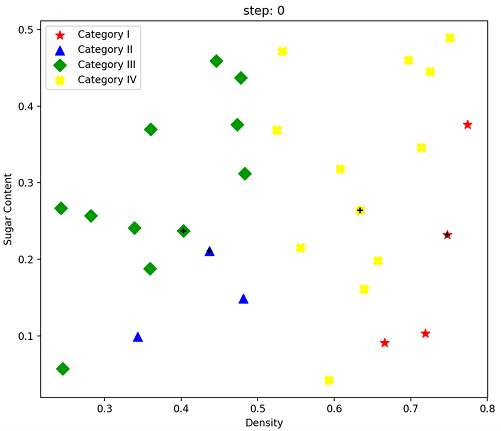
\includegraphics{Images/fig17.png}}
    \caption{Initial Situation}
    \label{fig17}
    \end{figure}

\begin{figure}[htb]
    \centerline{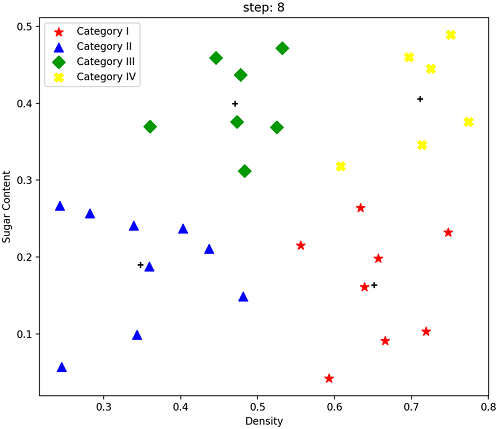
\includegraphics{Images/fig18.png}}
    \caption{Final Clustering Results}
    \label{fig18}
    \end{figure} \par
    \newpage

$\mathbf{Group 2}$:
\begin{figure}[htb]
    \centerline{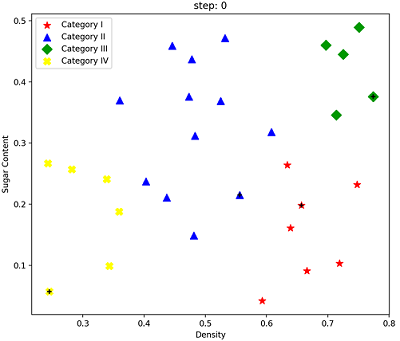
\includegraphics{Images/fig19.png}}
    \caption{Initial Situation}
    \label{fig19}
    \end{figure}

\begin{figure}[htb]
    \centerline{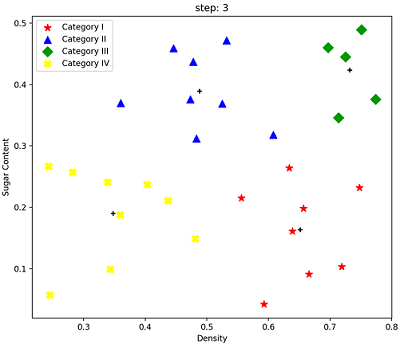
\includegraphics{Images/fig20.png}}
    \caption{Final Clustering Results}
    \label{fig20}
    \end{figure} \par

$\mathbf{Group 3}$:
\begin{figure}[htb]
    \centerline{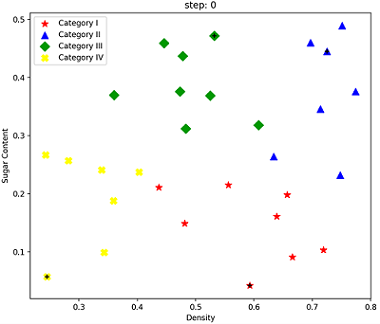
\includegraphics{Images/fig21.png}}
    \caption{Initial Situation}
    \label{fig21}
    \end{figure} 
    \vspace{20mm}
\begin{figure}[htb]
    \centerline{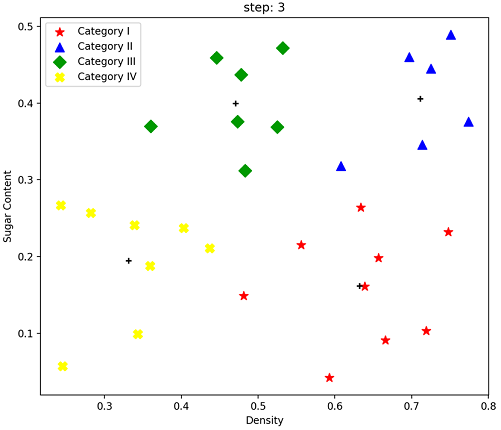
\includegraphics{Images/fig22.png}}
    \caption{Final Clustering Results}
    \label{fig22}
    \end{figure} \par

$\mathbb{A}2$:采用模糊$k-means$聚类的初始和优化后的隶属度矩阵如下图所示:
\begin{figure}[htb]
    \centerline{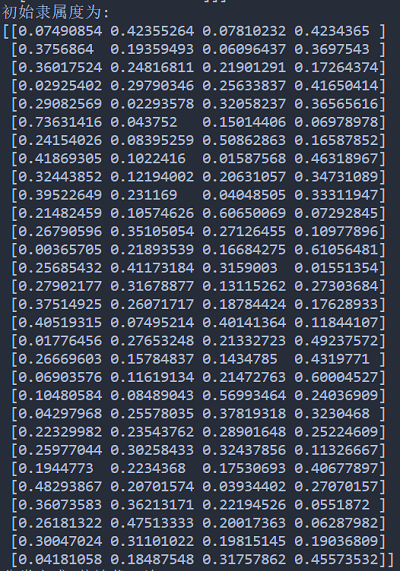
\includegraphics{Images/fig23.png}}
    \caption{Initial Membership matrix}
    \label{fig23}
    \end{figure} 

\newpage
\begin{figure}[htb]
    \centerline{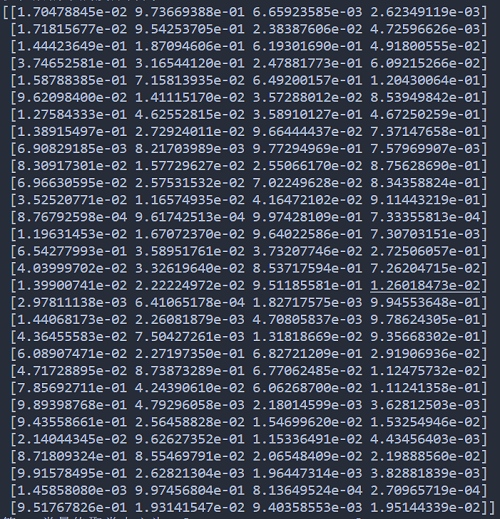
\includegraphics{Images/fig24.png}}
    \caption{Final Membership matrix}
    \label{fig24}
    \end{figure} \par
\end{CJK}
\end{document}
